\documentclass[a4paper, 12pt]{article}

\usepackage[T2A]{fontenc}
\usepackage[utf8]{inputenc}

\usepackage[english, russian]{babel}

\usepackage{amsmath, amsfonts, amsthm, mathtools, amssymb}
\usepackage[left = 1cm, top=10mm, right=20mm, bottom=0.6cm, bindingoffset=0cm]{geometry}
\usepackage{setspace}
\setstretch{1.2}
%Рисунки
\usepackage{graphicx}
\usepackage{wrapfig }
\usepackage{multirow}
\usepackage{booktabs}
\usepackage[table,xcdraw]{xcolor}
% Beamer presentation requires \usepackage{colortbl} instead of \usepackage[table,xcdraw]{xcolor}
\renewcommand{\arraystretch}{1.5}

\begin{document}
\begin{titlepage}
	\centering
	{\scshape\LARGE Московский физико-технический институт \par}
	\vspace{10cm}
	{\scshape\Large Лабораторная работа 3.4.4 \par}
	\vspace{1cm}
	{\huge\bfseries Петля гистерезизиса (статический метод) \par}
	\vspace{1cm}
	\vfill
\begin{flushright}
	{\large выполнили студент группы Б03-302}\par
	\vspace{0.3cm}
	{\LARGE Пазов Тенгиз, Симухин Егор}

\end{flushright}
	\vfill
% Bottom of the page
	04.11.2024 г.
\end{titlepage}
\large\section{Цель работы:}
\hspace{0.6cm} Наблюдение начальной кривой намагничивания ферромагнетиков и предельной петли гистерезиса

\section{Оборудование:}
\hspace{0.6cm} Источник питания, тороид, соленоид, баллистический гальванометр с осветителем и шкалой, амперметр, магазин сопротивлений, лабораторный автотрансформатор (ЛАТР), разделительный
трансформатор.

\section{Теоретические сведения:}
\hspace{0.6cm} Гистерезис - свойство систем, состояние которых зависит не только от значения внешних параметров, но от истории их изменений.
Гистерезис характерен для намагниченности ферромагнитного образца как функция напряженности магнитного поля в веществе M(H), но на практике магнитные свойства ферромагнетиков обычно изучают
путём измерения зависимости индукции магнитного поля B от напряжённости магнитного поля H в веществе.

Для кривой намагничивания вводится дифференциальная магнитная пронициаемость - наклон кривой намагничивания.
\begin{equation}
    \mu_{dif} = \frac{1}{\mu_0} \frac{dB}{dH}
\end{equation}

\begin{figure}[ht]
\begin{center}
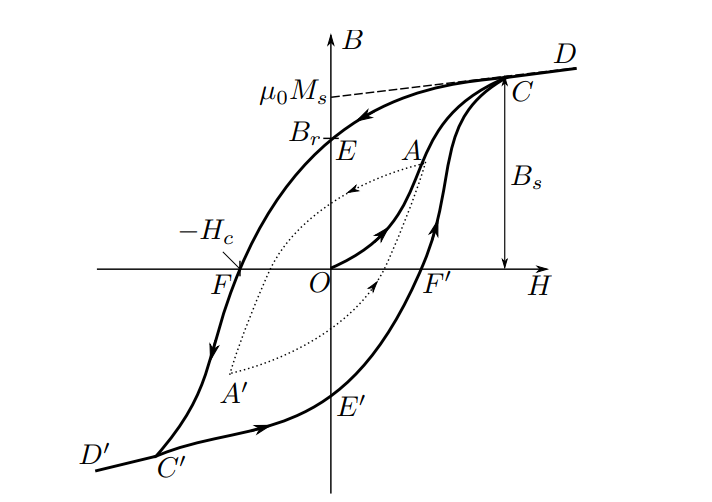
\includegraphics[width = 0.5\textwidth]{Снимок экрана 2024-11-27 235522.png}
\end{center}
\caption{Петля гистерезиса ферромагнетика}
\end{figure}


\subsection{Начальная кривая намагничивания}
Пусть ферромагнетик находится исходно
в ненамагниченном состоянии. Медленно увеличивая поле в
образце, получим зависимость, которую называют начальной кривой намагничивания (участок OAС).
В точке С намагниченность образца М  достигает насыщения и далее не зависит от H. Тогда индукция магнитного поля $B = \mu_0(H + M_{s}) = \mu_0 H + const$ зависит от H линейно.
При этом $M >> H$, тк для ферромагнетиков $M = \kappa H$. $\kappa$ - магнитная восприимчивость (не является константой и зависит от H) по абсолютному значению достигает значений $10^3 - 10^4$, поэтому $B = \mu_0(H + \kappa H) \approx \mu_0 \kappa H$, те кривая OAC практически совпадает с соответствующей зависимостью M(H) с точночтью до константы $\mu_0$.
Нетрудно видеть, что экстраполяция прямой CD до пересечения с осью ординат $H = 0$ позволяет определить намагниченность в насыщении $M_{s}$. В этом случае в СИ: 
\begin{equation}
    B = \mu_0(H + M_{s}) = \mu_0 M_{s}
\end{equation}

\subsection{Предельная петля гистерезиса}
Будем намагничивать ферромагнетик, дойдя таким образом до точки C. Пусть $H(С) = H_1$. Затем будем изменять H от $H_1$ до $-H_1$. Кривая намагничивания не пойдет по прежнему пути CAO, а пройдет выше, по пути DFC'. Легко видеть, что при $H = 0$ $B_{r}$ - остаточная индукция - не обращается в 0, а остается равным $B_{r}.
Тoгда:
\begin{equation}
    B_{r} = B(0) = OE
\end{equation}
В обращается в 0 при $H = -H_{c}$. Такое магнитное поле называется коэрцитивной силой ферромагнетика.
Тогда:
\begin{equation}
    H_{c} = H(0) = OF
\end{equation}
Далее будем изменять H от $-H_1$ до $H_1$. Кривая C'E'F' вернется в точку C.

\subsection{Принципиальный способ измерения}
\hspace{0.6cm} На тороидальный сердечник, изготовленный из исследуемого образца, равномерно намотана намагничивающая обмотка с числом витков N, а поверх неё - измерительная обмотка с числом витков N'. При скачкообразном изменении тока в намагничивающей обмотке в измерительной обмотке возникает ЭДС индукции. Ток, вызванный этой ЭДС, регистрируется гальванометром, работающим в баллистическом режимe.
Напряжённость поля H в сердечнике пропорциональна току I в
первичной (намагничивающей) обмотке, а изменение магнитной индукции $\Delta B$ — заряду $\Delta q$, протекшему через измерительную обмотку. Таким образом, измеряя токи I и суммируя отклонения $\Delta q$ гальванометра, можно получить зависимость B(H) для материала сердечника.

\subsection{Измерение полей}
Напряженность магнитного поля тороида:
\begin{equation}
    H \approx \frac{N}{\pi D} I
\end{equation}
где D — средний диаметр тора.

Связь магнитной индукции с отклоением первого отброса зайчика гальванометра:
\begin{equation}
    \Delta x = \frac{\pi D^2 N'}{4bR} \Delta B
\end{equation} 
где R - полное сопротивление измерительной цепи тороида, b - баллистическая постоянная гальванометра.

Тогда остается лишь найти баллистическую постоянную.
Для этого проведем аналогичные измерения, взяв вместо тороида с сердечником пустотелый соленоид с числом витков $N_{c}$, на который намотана короткая измерительная катушка с числом витков $N_{c}$'. Для длинного пустого соленоида
имеем:

\begin{equation}
    B_{c} = \mu_0 H_{c} = \frac{N_{c}}{l_{c}} I
\end{equation}
где $l_{c}$ — длина соленоида.

Показания гальванометра при изменении тока в соленоиде:
\begin{equation}
    \Delta x = \frac{\pi D_{c}^2 N_{c'}}{4bR_{c}} \Delta B_{c}
\end{equation}

Исключая b из уравнений для $\Delta x$:
\begin{equation}
    \Delta B = \mu_0 N_{C} \frac{N_{c}'}{N'} \frac{R}{R_{c}} \frac{d_{c}^2}{d^2} \frac{\Delta I_{c}}{l_c} \frac{\Delta x}{\Delta x_{c}}
\end{equation}

\subsection{Размагничивание образцов}
Для размагничивания ферромагнитных объектов используют метод с постепенным уменьшением амплитуды переменного тока. Ферромагнетик помещают в катушку, через которую пропускают переменный ток. Постепенно уменьшая амплитуду тока, ферромагнетик подвергают циклическому перемагничиванию. В этом процессе возникают всё более узкие петли гистерезиса, что постепенно снижает остаточное намагничивание ферромагнетика. В итоге объект достигает состояния, в котором намагниченность полностью исчезает.

\section{Экспериментальная установка}

Детальная схема измерений петли гистерезиса представлена на
рис. 2. К блоку питания (источнику постоянного напряжения) подключён специальный генератор, позволяющий скачками менять токи в намагничивающей обмотке.
Ток в намагничивающей обмотке измеряется амперметром. Переключатель П1 позволяет менять направление тока в первичной обмотке.
Чувствительность гальванометра Г во вторичной цепи можно менять
с помощью магазина сопротивлений $R_{M}$. Ключ К2 предохраняет гальванометр от перегрузок и замыкается только на время измерения отклонений зайчика. Ключ К0 служит для мгновенной остановки зайчика (короткое замыкание гальванометра). Переключатель П1 позволяет менять направление тока в первичной обмотке. Переключателем П2 можно изменять направление тока через гальванометр. Ток в намагничивающей обмотке измеряется амперметрами А1 и A2 с разными пределами
измерения.
Схема на рис. 3 отличается от схемы на рис. 2 только тем, что вмест тороида подключён калибровочный соленоид.

\begin{figure}[!h]
\begin{center}
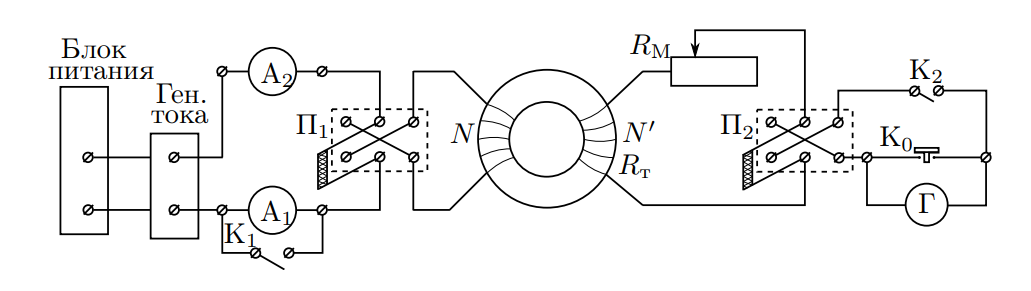
\includegraphics[width = 1\textwidth]{Снимок экрана 2024-11-27 235648.png}
\end{center}
\caption{Схема установки для исследования петли гистерезиса}
\end{figure}

\begin{figure}[!h]
\begin{center}
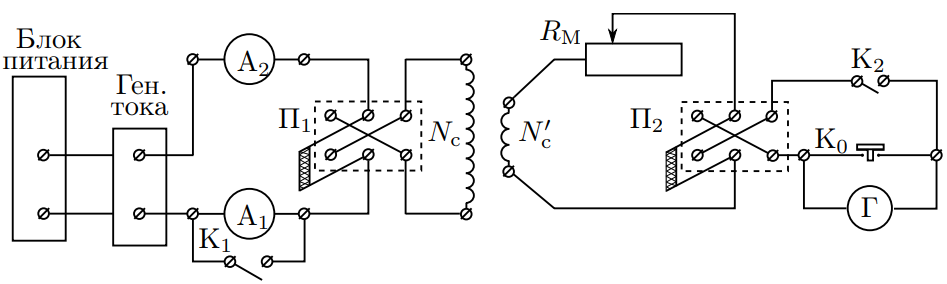
\includegraphics[width = 1\textwidth]{Снимок экрана 2024-11-27 235740.png}
\end{center}
\caption{ Схема установки для калибровки гальванометра}
\end{figure}

Чтобы снять начальную кривую
намагничивания, нужно предварительно размагнитить образец.
Для этого тороид подключается
к цепи переменного тока (рис. 4).
При уменьшении амплитуды
тока через намагничивающую
обмотку от тока насыщения до нуля характеристики сердечника B
и H «пробегают» за секунду 50 петель всё меньшей площади и в итоге
приходят в нулевую точку.

\begin{figure}[!h]
\begin{center}
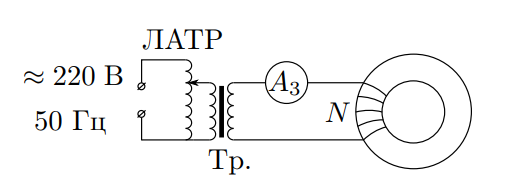
\includegraphics[width = 0.6\textwidth]{Снимок экрана 2024-11-28 000333.png}
\end{center}
\caption{Схема размагничивания}
\end{figure}
\section{Ход работы}
\subsection{Построение кривой гистерезиса}
\begin{itemize}
    \item На схеме, собранной согласно рис 3, установим значение сопротивления на магазине сопротивлений $R_{M} > R_{c}$ и, начиная с максимального тока намагничивания, будем отмечать величину I, соответствующую каждой позиции тумблера генератора, и отклонение зайчика, соответствующие каждому щелчку. По этим данным получим зависимости $H(I)$ и $B(\Delta x)$
    \item Затем определим баллистическую постоянную гальванометра. Для этого заместо тороида подключим соленоид, изменим сопротивление на магазине сопротивлений на значение $R = R_{M} - R_{c}$ и, установив тумблер генератора на максимум, запишем значение тока и отклонение гальванометра
    \item Размагнитим образец с помощью схемы на рис 4
    \item Снова подключим тороид к схеме 2. Будем скачами изменять ток с 0 до максмального и снимать отклонение зайчика. Так мы получим данные для начальной кривой гистерезиса
    \item Затем построим кривую гистерезиса $B(H)$. Просуммируем все скачки $\Delta B$ и $\Delta x$, найдем середину петли и проведем ось $H(I)$ и $B(\Delta x)$
    \item Построим начальную кривую намагничивания на этом же графике
    \item Аппроксимируя прямыми зависимость $B(H)$ для соседних точек, найдем точки пересечения кривой гистерезиса с осями - так получим коэрцитивное поле $H_{c}$, остаточную индукцию $B_{r}$ и индукцию насыщения $B_{s}$
    \item Выделяя линейный участок при $H > H_{s}$ и экстраполируя его до пересечения с осью ординат $H = 0$, найдем максимальную намагниченность $M_{s}$
    \item Определим максимальное значение дифференциальной магнитной проницаемости $\mu_\text{dif}$, проведя касательную к графику в области с наибольшим наклоном начальной кривой намагниченности
\end{itemize}

\subsection{Результаты и оценка погрешностей}

\begin{table}[!h]
\centering
\begin{tabular}{@{}|
>{\columncolor[HTML]{DCDCDC}}l |l|l|l|@{}}
{\color[HTML]{C0C0C0} } & \cellcolor[HTML]{DCDCDC}Значение    & \cellcolor[HTML]{DCDCDC}Погрешность  & \cellcolor[HTML]{DCDCDC}Табличные значения  \\ \midrule
$H_{c}$                 & 288.8 А/м                           & 28.84 А/м                             & 240.0 А/м                          \\ \midrule
$B_{r}$                 & 0.43 Тл                              & 0.003 Тл                               & 0.8 Тл                         \\ \midrule
$B_{s}$                 & 0.47 Тл                              & 0.006 Тл                               & -                          \\ \midrule
$M_{s}$                 & 3.8 * 10\textasciicircum{}(5) А/м   & 0.9 * 10\textasciicircum{}5 А/м      & -                          \\ \midrule
$\mu_\text{dif}$        & 761.95 м Тл / А                        & 36.86 м Тл / А                          & -                       \\ \bottomrule
\end{tabular}
\end{table}

\begin{itemize}
    \item При определении точки пересечения графика с осью абсцисс будем аппроксимировать точки в окрестности нуля прямой по мнк, считать погрешность аналогично
    \item Для погрешности точки пересечения графика с осью ординат и для погрешности максимальной намагниченности $M_{s}$ будем использовать погрешность определения B:
\begin{equation}
    \sigma_{B} = B \varepsilon_{\Delta x}
\end{equation}
где $\sigma_{x} = 0.5$ см
    \item При определении максимального значения дифференциальной магнитной проницаемости $\mu_\text{dif}$, будем использовать МНК
\end{itemize}

\begin{figure}[h!]
\begin{center}
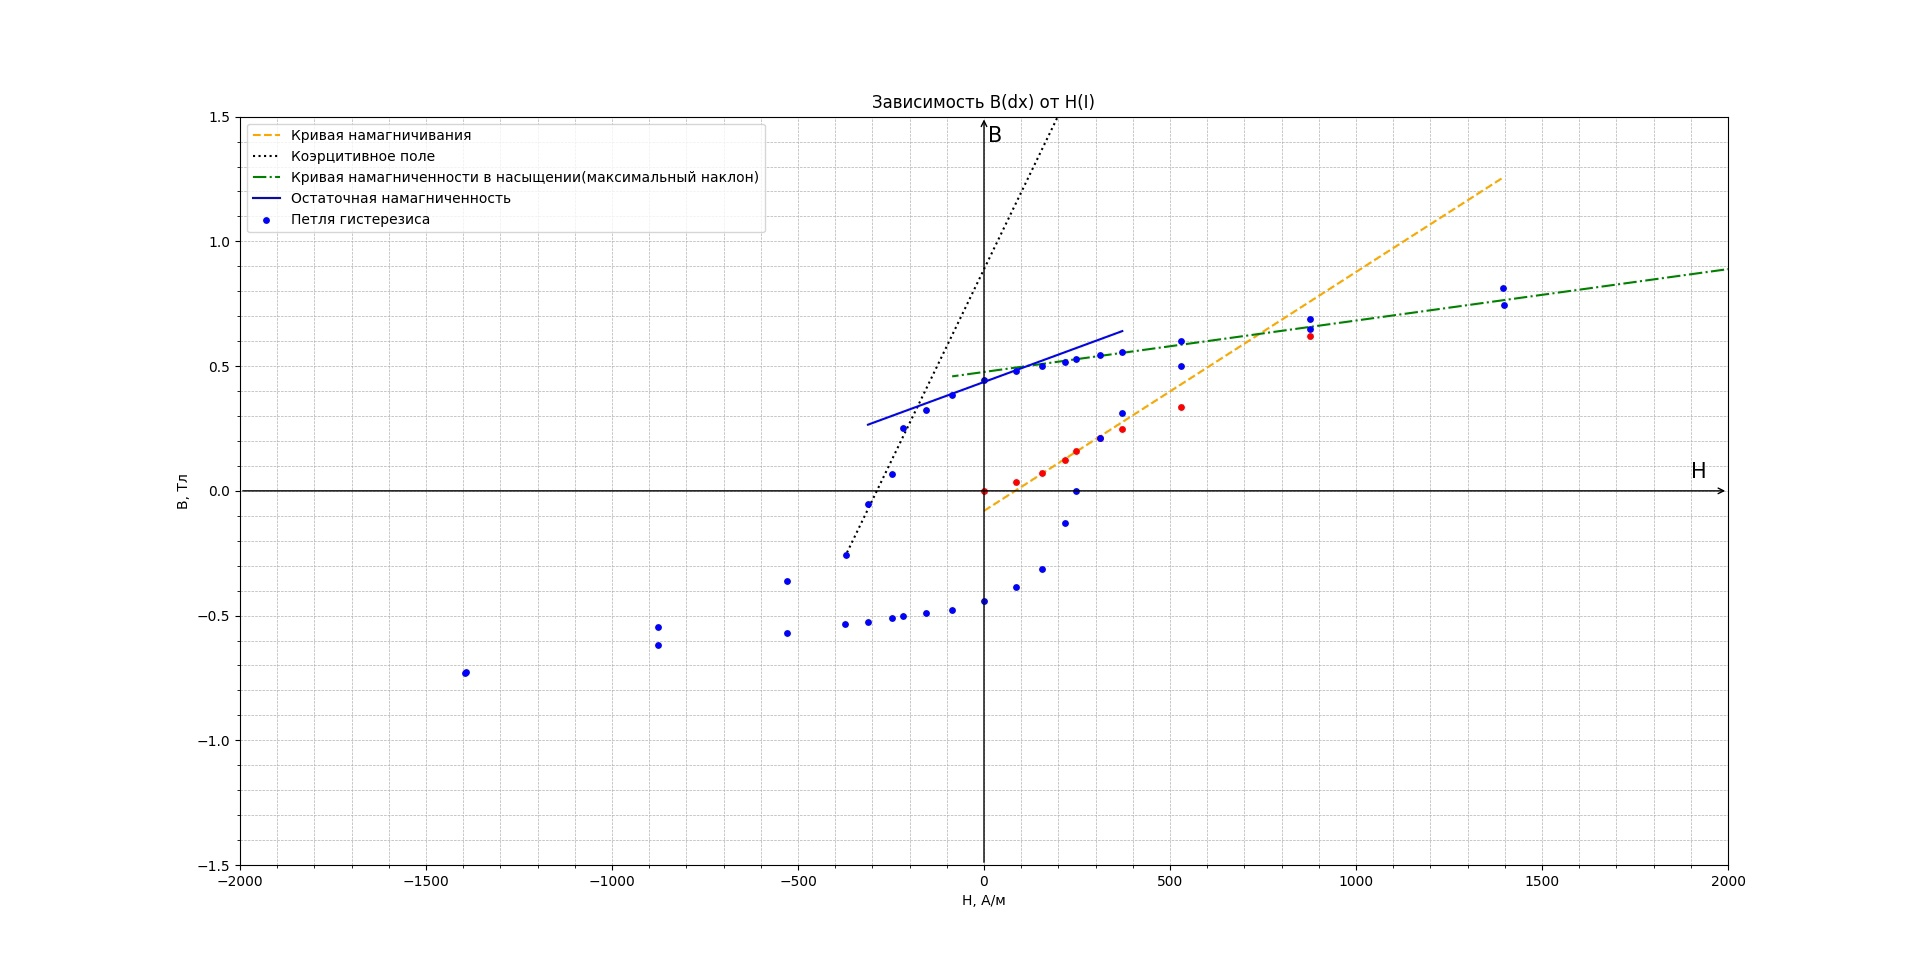
\includegraphics[width = 1.2\textwidth]{TMf2sm6-Q9Y.jpg}
\end{center}
\caption{Кривая гистерезиса}
\end{figure}
Также были получены координаты точки касания: H = 228 А/м, B = 0.128 Тл

\newpage
\section{Вывод}
\hspace{0.6cm} В данной работе был рассмотрен гистерезис ферромагнетиков, получены предельная кривая намагничивания, начальная кривая намагничивания. Полученная предельная кривая симметричная. Были получены различные характеристики ферромагнетика - коэрцитивное поле $H_{c}$, остаточная индукция $B_{r}$, индукция насыщения $B_{s}$, максимальная намагниченность $M_{s}$ и максимальное значение дифференциальной магнитной проницаемости $\mu_\text{dif}$.

\end{document}
